%%%%%%%%%%%%%%%%%%%%%%%%%%%%%%%%%%%%%%%%%
% University Assignment Title Page 
% LaTeX Template
% Version 1.0 (27/12/12)
%
% This template has been downloaded from:
% http://www.LaTeXTemplates.com
%
% Original author:
% WikiBooks (http://en.wikibooks.org/wiki/LaTeX/Title_Creation)
%
% License:
% CC BY-NC-SA 3.0 (http://creativecommons.org/licenses/by-nc-sa/3.0/)
% 
% Instructions for using this template:
% This title page is capable of being compiled as is. This is not useful for 
% including it in another document. To do this, you have two options: 
%
% 1) Copy/paste everything between \begin{document} and \end{document} 
% starting at \begin{titlepage} and paste this into another LaTeX file where you 
% want your title page.
% OR
% 2) Remove everything outside the \begin{titlepage} and \end{titlepage} and 
% move this file to the same directory as the LaTeX file you wish to add it to. 
% Then add \input{./title_page_1.tex} to your LaTeX file where you want your
% title page.
%
%%%%%%%%%%%%%%%%%%%%%%%%%%%%%%%%%%%%%%%%%
%\title{Title page with logo}
%----------------------------------------------------------------------------------------
%	PACKAGES AND OTHER DOCUMENT CONFIGURATIONS
%----------------------------------------------------------------------------------------

\documentclass[12pt,twocolumn]{article}
\usepackage[english]{babel}
\usepackage[utf8x]{inputenc}
\usepackage{amsmath}
\usepackage{graphicx}
\usepackage[colorinlistoftodos]{todonotes}
\usepackage{pifont}
\usepackage{skull}
\usepackage{wasysym}
\usepackage{skak}
\usepackage{hyperref}
\usepackage{enumitem}
\usepackage{systeme}

\begin{document}

\begin{titlepage}

\newcommand{\HRule}{\rule{\linewidth}{0.5mm}} % Defines a new command for the horizontal lines, change thickness here

\center % Center everything on the page
 
%----------------------------------------------------------------------------------------
%	HEADING SECTIONS
%----------------------------------------------------------------------------------------

\textsc{\LARGE Università degli studi di Milano-Bicocca}\\[1cm] % Name of your university/college
\textsc{\Large Decision Models}\\[0.3cm] % Major heading such as course name
\textsc{\large Final Project}\\[0.1cm] % Minor heading such as course title

%----------------------------------------------------------------------------------------
%	TITLE SECTION
%----------------------------------------------------------------------------------------

\HRule \\[0.4cm]
{ \huge \bfseries Methodological approaches for Multi-agent RL games}\\[0.4cm] % Title of your document
\HRule \\[1.5cm]
 
%----------------------------------------------------------------------------------------
%	AUTHOR SECTION
%----------------------------------------------------------------------------------------

\large
\emph{Authors:}\\
Riccardo Cervero - 794126\\   
Federico Moiraghi - 799735\\ 
Pranav Kasela - 846965\\[1cm] 
%----------------------------------------------------------------------------------------
%	DATE SECTION
%----------------------------------------------------------------------------------------

{\large \today}\\[2cm] 

%----------------------------------------------------------------------------------------
%	LOGO SECTION
%----------------------------------------------------------------------------------------


\includegraphics[width=0.2\textwidth]{./figs/logo.png}\\[1cm] 
%----------------------------------------------------------------------------------------

\vfill % Fill the rest of the page with whitespace

\end{titlepage}


%\begin{abstract}
%The purpose of this project is to create systems able to simulate human behaviors and tendencies when subjected to incentives within different environments. 
%In 4 games, agents will establish mutual relations, fostered by positive or negative signals, and natural factors such as the health and fear level will be recreated. 
%More precisely, in the first experiment three different methods will be used to allow a single Reinforcement Learning system to beat a non-intelligent rival. 
%In the next two, the players will be pushed to face each other in a fight, configured first as a duel and then as a battle - among five of them. Finally, two players will be encouraged to act together to eliminate a common enemy.\\*
%Each game is accompanied by a graphic component that shows the actual progress of the game.\\*
%\end{abstract}
%\newpage
\newpage
\tableofcontents
\newpage
\section{Introduction}
Reinforcement Learning is the branch of Machine Learning gathering several techniques designed to create a system, an agent, capable of learning the best way to achieve goals within an environment, whose elements - such as, for example, obstacles or objectives - can also vary over time. In other words, this agent simulate the process of human understanding, by exploring the initially unknown environment and consequently receiving rewards or penalization based on the goodness of the choices made.\\*
The goals of this project are:
\begin{enumerate}[noitemsep, topsep=0ex]
	\item Using different methodologies to perform the same Reinforcement Learning experiment (Game 1);
	\item Deepening the dynamics among multiple separate agent, each of which will learn automatically and independently how to win the game by looking and reacting to other agents' choices. In particular, the two dynamics of ``competition'' and ``cooperation'' will be examined.
\end{enumerate}
To do so, four ``worlds'' have been built, with different rules and components - such as fear or randomly moving obstacles -, within whom the agents will be trained over several epochs to maximize the reward, beat the rivals or help the allies in the best way possible.\\*
The following sections will present games' and agents' characteristics.
\newpage

\section{Game 1: Bilbo and the dragon}
This first experiment has been created with the aim of employing Q-Learning algorithm, a Deep Q-Learning approach and Deep Q-Learning with the integration of Genetic Algorithm on a single system whose objective is beating a non-intelligent rival.\\*
The environment in which the three Bilbos will be trained within is defined as a class named ``World''\footnote{\href{https://github.com/moiraghif/DragonHunting/blob/master/Bilbo\%20World/CreateBilboWorld.py}{Link to the code here.}}, which is a 15x15 array, to which various elements are added:
\begin{itemize}[noitemsep, topsep=0ex]
  \item Optional \textbf{obstacles}, randomly generated with a seed, so their position is randomly chosen but will remain the same throughout the games;
  \item A non movable \textbf{treasure}, which can be located in a randomly chosen coordinate or predefined too. It can only caught by the agent;
  \item A \textbf{dragon}, which represents the non-intelligent enemy of the agent.
  \item \textit{\textbf{Bilbo}}, the agent to be trained, which is always generated at a random position. Unlike the other components, Bilbo moves around the world trying to maximize the total reward of his game and avoid penalties in best way possible, which is the core operating principle of any Reinforcement Learning methodology.
\end{itemize}
Therefore, Bilbo's goal is to reach the cell where the treasure is without getting caught by the dragon, condition that occurs when the two end up in the same cell. The game ends when Bilbo is killed by the dragon in the terms just described, or when he manages to get the treasure, escaping from the enemy among the obstacles scattered around the world. The reward is based on every game state:
\begin{itemize}[noitemsep, topsep=0ex]
  \item If Bilbo reaches the treasure, he gets a positive reward of 15;
  \item If Bilbo has been killed by the dragon, he gets a penalty of -15;
  \item At each moves, Bilbo receives a penalty of -1. This negative reward serves to incentivize Bilbo to find shorter routes to reach the treasure. Another strategy, used in combination with a Deep Q-Learning approach, consists in offering a positive reward of +1 when Bilbo gets near the treasure, and -2 otherwise, in order to make the convergence of the method faster
  \item If Bilbo dumps into an obstacle, so his position remains the same, he gets a penalty of -5, so that he learns to avoid them
\end{itemize}
Another Python class named ``Agent''\footnote{\href{https://github.com/moiraghif/DragonHunting/blob/master/Bilbo\%20World/agents.py}{Link to the code here.}} serves to set the main characteristics of Bilbo.
He can move in the same four direction of the dragon - `up', `down', `right', `left'. \\*
He is affected by a ``fear'' factor, in order to simulate an aspect of real human exploring process. If Bilbo is far from it, the ``fear'' value is close to 1; otherwise, as the distance from the dragon decreases, the value increases at most to 2. This measure is calculated as follows: 
$$\Big(\frac{d}{1+d}\Big)^{-1}$$
with $d$ representing the Euclidean distance between the dragon's position and Bilbo's location.
This will consist in a divisor of the $\varepsilon$ parameter used in Reinforcement Learning algorithms to produce random moves in the grid and allow a better exploration of the world. As one can see from the formulation, this factor is a normalized distance, used to prevent $\varepsilon$ to be too much affected by it.\\*
In conclusion, in this way, when Bilbo approaches the dragon, his fear level increases and the chance of a random exploration as well.

Given this general aspects of Game 1, three methodologies have been exploited to provide the agent with a learning process, each based on an agent generalization provided by a new Python class.

\subsection{Q-Learning algorithm}
The first approach consists in Q-Learning algorithm\footnote{The code consists in QLearningAgent class in \href{https://github.com/moiraghif/DragonHunting/blob/master/Bilbo\%20World/agents.py}{this file} and also \href{https://github.com/moiraghif/DragonHunting/blob/master/Bilbo\%20World/Bilbo_q_learning.py}{the scripts inside this file}.} \cite{2}, which is based on the propagation of potential reward from the best possible actions in future states. Following this idea, each action in each state is related to a Q value, updated when new relevant information about the environment, derived from exploration, is made available. The Q-Learning algorithm utilizes the following updating rule:
$$Q(s,a)=$$ 
$$Q(s,a)+\alpha(r+\gamma\;max\;Q(s',a') - Q(s,a))$$
with $Q(s,a)$ Q-value of current state and $Q(s',a')$ Q-value of next state; $r$ the reward obtained by taking action $a$ at the state $s$; $\gamma$ discounting factor regulating the impact of future rewards; $\alpha$ learning rate. In this case, the values of the hyper-parameters chosen were $\alpha=0.5, \gamma=0.8$, and $\varepsilon=0.2$\\*
Hence, the worth of an action in a certain state also depends on the discounted worth produced by the best action in the next state $s'$, and on the extent of the steps to the convergence selected with parameter $\alpha$. In other words, this policy makes agent estimate the goodness of an action in a certain state based on the cascaded, discounted reward from the next states, where the states, in this case, are given only by Bilbo's coordinates. 
In this way, at state $s$, Bilbo will not choose the action providing the best rewards only in the current state, but the action which leads to the best total rewards over all the states, while exploring the world in order to discover the rewards or penalties of all action. As Q-values are updated, they are stored in a Q matrix\footnote{Q-matrices are available \href{https://github.com/moiraghif/DragonHunting/tree/master/Bilbo\%20World/models}{here.}}, so that Bilbo can learn from past experiences. This exploration process, that consists merely in random moves around the ``gridworld'', is fostered by $\varepsilon$ parameter, which depends on ``fear factor'' as aforementioned. More over, $\varepsilon$ decays by being multiplied to a ``decay factor'' (of $0.99$) at each step, up to a minimum of $0.01$.\\*
In conclusion, this process can be explained as follows: if a number extracted from a uniform between 0 and 1 is less than $\varepsilon$, the system performs a random step. Otherwise, it performs the action related to the maximum Q value in that state.\\* 
Then, the limits of epochs and episodes executable are both set to 2000.\\*
During the iterations, the performances of Bilbo are tracked by counting the number of wins, cases where he manages to stay alive and get the treasure, and losses, when he ends up killed by the dragon.

\subsection{Deep Q-Learning (DQL) approach}
In the previous methodology, Q-Learning algorithm, the experience acquired by Bilbo during the games was based on explicit tables, - Q matrix and reward matrix - holding the information discovered. This tables could end up to be far too large and unwieldy when the game is composed of a large number of states and potential actions, or the world becomes larger.\\*
The solution to this problem can be the application of a Deep Reinforcement Learning methodology \cite{3,6}, which consists in training a neural network to predict Q values for each action in a certain state, instead of having explicit tables.\\*
The spawn of Treasure and Dragon is completely random and the obstacles are no more present.
Each time the treasure is collected by Bilbo, it respawns randomly on the map.
As far as neural network, implemented within Q-learning algorithm, the input is not only the simple set of coordinate describing the location of the agent, the dragon and the treasure, but a more general from, so that the model will be able to generalize to different scenarios. This reshaped form of current state is produced by:
\begin{enumerate}[noitemsep, topsep=0ex]
  \item computing the relative position between Bilbo and the treasure and between Bilbo and the dragon by subtracting respective coordinates;
  \item checking whether the position of Bilbo is at the border for all four sides - ordered as ``up'', ``down'', ``right'', ``left'' - and assigning 0 if the given direction is accessible or 1 if it is borderline.
\end{enumerate}
After this transformation, the current state that will form the input of the neural network will appear as an array containing the two relative coordinates and the aforementioned binary values. For example, if Bilbo were on the leftmost edge of the gridworld, the input neurons would receive the following elements:
$$
[B_{(x,y)}-T_{(x,y)},\;B_{(x,y)}-T_{(x,y)},\;0,\;0,\;0,\;1]
$$
The output are the Q values for each action in the given state, which will approach the results produced by the learning update previously utilized. Therefore, using the mean-squared error metrics, the loss or cost function for the neural network will be:
$$(r+\gamma\;max_{a'}\;Q'(s',a')-Q(s,a))^2$$
Starting from this, the neural network is built as a sequential model composed by:
\begin{itemize}[noitemsep, topsep=0ex]
  \item the input layer of 8 neurons, receiving the reshaped current state, namely the information about the relative position of the other entities and with respect to the border;
  \item an hidden layer composed by 16 neurons activated by a Rectified Linear Unit (ReLU) function; 
  \item the linear activated output layer with one neuron for each possible action in the given state, which hence performs the linear summation of the inputs and the weights providing the estimated Q values.
\end{itemize}
The model is compiled using the aforementioned mean-squared error loss function and the Adaptive Moment Estimation as optimizer.\\*
As Bilbo explores the world, his experience is described into 5 values: current state, action, reward, next state and game state. Since, among all the moves performed, the probability that one of them leads to Bilbo's victory - attainment the treasure - or to his defeat - capture by the dragon - is very low, two separate memories are established: one dedicated to the unlikely events just defined, the other storing the rewards obtained in the normal phases of the game. Therefore, when the system has developed sufficient experience in the world, in order to calculate the exact Q-values for each action in the given state, at each epoch the model is trained on a \textit{mini-batch} consisting of the union of 32 elements randomly extracted respectively from both separate memories. While the system performs these steps, it simultaneously updates the Q-values\footnote{\href{https://github.com/moiraghif/DragonHunting/blob/master/Bilbo\%20World/Bilbo_deep_feels.py}{The code is available here} and in the ``DeepQLearningAgent'' class \href{https://github.com/moiraghif/DragonHunting/blob/master/Bilbo\%20World/agents.py}{described inside this file}.}.\\*
As before, performances, computed by the number of win and losses, are tracked over the 20000 episodes, which involve at most 150 epochs.\\*
The hyperparameters are:
$\gamma$ = 0.8, maintaining the same Bilbo's ``foresight'' as before,
$\varepsilon$ = 0.5, increasing the fixed component of random exploration probability with respect to the previous section and
$decay\;factor$ = 0.9998, further slowing the decay\\*
Model training required $\sim$19 hours with more that 2 million steps, in the testing phase. The model achieved an average reward of 300 over 1000 episodes (See Figure~\ref{fig:deep_vs_ga}).

\subsection{Genetic Algorithm}

An issue that needs to be further investigated to achieve accurate estimation performances through a neural network is the tuning of learning parameters involved in the training process. In the previous section, the optimization technique used for updating the weights of the sequential model was the Adaptive Moment Estimation. This one consists in an extension of Stochastic gradient descent method (SGD), considered as standard \textit{de facto} for training artificial neural networks. However, despite its properties, it can be replaced by other methodologies, including the class of metaheuristics called evolutionary algorithms (EA). The main difference between SGD and EA lies in the fact that the second ones are well suited for multi-criteria optimization, when gradient descent is dedicated to mono-criteria optimization.\\*
A solution part of the EA class is represented by the Genetic Algorithm \cite{7}, which simulates the evolution of an initial population towards the best possible solution, the typical mechanism of the natural selection. During this process, each candidate solution present in the initial population of randomly generated individuals has a set of properties, chromosomes or genotype, which can be mutated and altered. 
Therefore, in this third subsection, Genetic Algorithm will be presented as an alternative, search-based, optimization method for learning weights within the Deep Reinforcement Learning system.\\*
The operation mode of this third algorithm\footnote{\href{https://github.com/moiraghif/DragonHunting/blob/master/Bilbo\%20World/Bilbo_ga_deep_feels.py}{The code is available here} and in the ``DeepQLearningAgentGA'' class \href{https://github.com/moiraghif/DragonHunting/blob/master/Bilbo\%20World/agents.py}{inside this file.}} is completely identical to the previous one, except for the use of GA within the neural network training process. The neural network is simplified by removing the hidden layer. 
In details, the weights optimization process takes place as follows: the system initializes 150 random sets of weights, Bilbo's learning parameters, and evaluates the fitness of every individual within each generation, where the fitness is the average reward collected over 3 games - here the objective is to maximize the fitness -, returning the individuals sorted according to their score. From them, it extracts the first 10\% - elitism parameter -, which will be used as parents of next generation. Indeed, each new individual will be created with a crossover function which randomly chooses among the genes of two parents, considered as ``father'' and ``mother''. After eventually undergoing a random mutation process - the multiplication of genotypes, hence the value of each weight, by a random number between -2 and 2 - , with a probability set equal to 5\%, these ``children'' are in turn used to produce a new generation. When 150 generations have been produced - iterations stopping criterion -, the algorithm obtains a certain solution for the weights values, which are finally passed to the neural network. \\*
The training required $\sim$3 hours (6-7 times faster than Deep Q-Learning) and the average score of the trained model, over 1000 episodes, was 360, slightly higher that the Deep Q-Learning Method (See Figure~\ref{fig:deep_vs_ga}).

\begin{figure}[!h]
	\vspace{-2cm}
	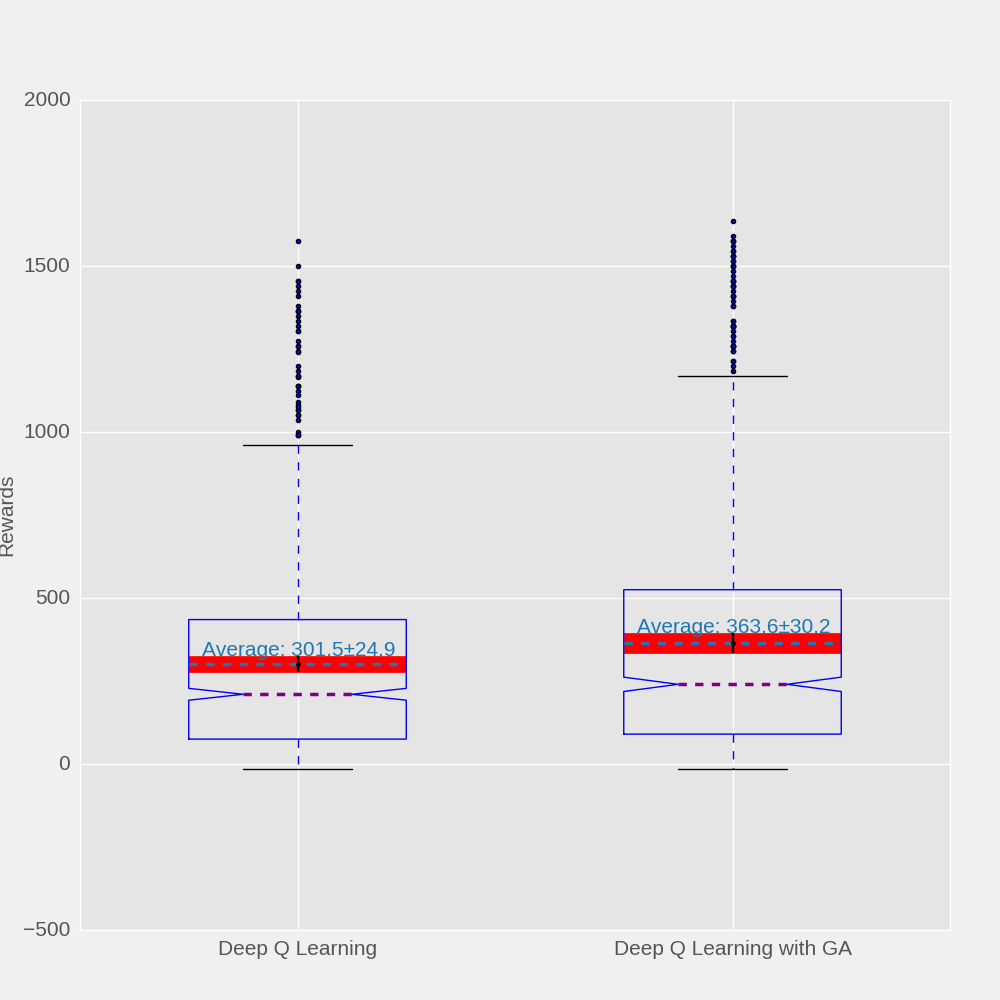
\includegraphics[width=\linewidth]{./figs/deep_vs_ga.png}
	\vspace{-1.5cm}
	\caption{Comparison of the results of DQL and DQL with GA over 1000 games}
	\label{fig:deep_vs_ga}
	\vspace{-0.5cm}
\end{figure}

\section{Multi-agent Competition}
As mentioned above, the second objective is the study of competition dynamics between independent agents. This in-depth analysis is the result of two games characterized by a different complexity from the conceptual and technical point of view. Therefore two new worlds are built, and agents competing within them will be based on a Q-Learning algorithm, without any Deep Reinforcement Learning generalization or alternative optimization methods, so as not to further increase the intricacy distinguishing these experiments.
\subsection{Game 2: Duel between two agents}
In Game 2\footnote{\href{https://github.com/moiraghif/DragonHunting/tree/master/Duel}{Link to the code here.}}, two players learn how to avoid fixed walls scattered in the grid and how to choose the best moment and way to approach and attack the opponent, in a duel where only one winner is allowed. There are two rivals, whose locations are randomly initialized, and the obstacles randomly situated as well. 
The ``Agent'' can perform the following actions: `up', `down', `left', `right' and `attack'. The attack is able to inflict damage only when rival's position is close enough. When one of them is hit, he suffers a reduction in his so-called ``health'' parameter, which is initially set at 10 points. The reward are set as follows:
\begin{itemize}[noitemsep, topsep=0ex]
  \item If a player carries out an attack at a distance that is less than 1, makes other agent's health score decrease by one point and this opponent receive a negative reward of -1 for the next move, while the player receives a reward of 10;
  \item If after 500 epochs, when the game ends, the rival's health score is higher than 0, then the player receives a 10 point penalty.
\end{itemize}
In this way, the agent is encouraged to approach and attack as soon as the distance becomes short enough, despite the fact that he himself could be injured, since the signal received if the other one had residual health at the end of the game is much more negative with respect to the penalty received at each stroke suffered. Therefore, after having explored the world and developed sufficient experience in the various episodes, the two players will tend to face each other, without ``fearing'' the clash. If, on the other hand, the penalty in case of damage suffered was higher, the two agents could have preferred the escape, which means they would have limited themselves to move away from the opponent and maintain the distance beyond the unit in absolute value.\\*
The operation mode is similar to the normal Q-learning algorithm, exception made for the way the two agents learn how to win the game: while Bilbo was limited to acquire the right way to avoid an element that performed random movements, the dragon, and reach the treasure, in this experiment the duelists will be forced to react to the opponent's moves and choose the right moment to attack. At each step, if a number randomly extracted from a uniform variable is less than $\varepsilon$ hyperparameter ($=0.05$), one system performs a random moves among the five possibilities, otherwise, it chooses the action maximizing the Q-value by looking at the Q-matrix entries in correspondence with current state, which is composed of its position and the opponent's coordinates.\\*
The game will be repeated 100,000 times. The hyperparameters of both duellists are set as follows: the discount factor $\gamma = 0.9$, the learning rate $\alpha = 0.75$

\subsection{Game 3: Battle among five agents}
This third experiment\footnote{\href{https://github.com/moiraghif/DragonHunting/tree/master/Duel_2}{Link to the code here.}} is configured as an extension of the previous game, in which 5 players will wander around the world and will be pushed, still by tuning the various penalties, to eliminate each other in a battle all against all, a Battle Royale. 
At this point, the current state, would have 10 dimensions, i.e. 2 coordinates for each of the 5 players. Therefore, every player's Q-matrix would have an excessive dimensionality ($5\cdot20^{10}$), forcing the Q-learning algorithm to calculate the distance and the direction based on each of the 10 coordinates. 
In order to avoid such a computational weight, a technical improvement has been introduced: the conversion of the initial gridworld into a graph. 
By replacing the empty cells with a node, based on the positions of the predetermined obstacles, and combining these with edges to delineate the accessible paths (See Figure \ref{fig:world2graph}), it is possible to exploit a clearly more efficient method for calculating the distance: the shortest path. 
In details, during each epoch, with the purpose of being able to ``observe'' the moves of the adversaries within the environment, in order to react to them in a reasonable time, which means evaluating the current state and opt for the action that maximizes the q-value of the given state, each system, instead of normally monitoring the proximity of the others through the coordinates, gets the fastest route to reach every other character in the game by formulating a ``shortest path'' problem. 
Finally, the direction of the vector towards which the closest enemy is situated is calculated. 
This approach greatly reduces the time required for the computation of a given state, thereby decreasing the total duration of the learning process. Thanks to the new structure, the current status consists of only 2 values for each precise opponent:
\begin{itemize}[noitemsep, topsep=0ex]
  \item the direction - between the usual 4 - towards which the player must move to reach the closest rival,
  \item a binary number equal to 0 if the distance between players and the closest enemy is null, that is when the players are in adjacent positions, and 1 otherwise.
\end{itemize}

\begin{figure}
	\centering 
	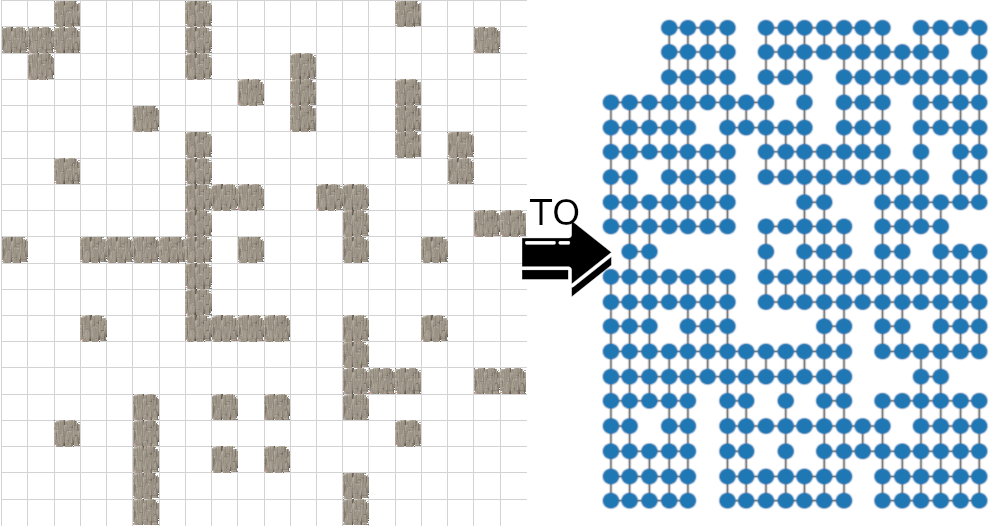
\includegraphics[width=\linewidth]{./figs/World2graph.png}
	\caption{Conversion from a Gridworld to a Graph}
	\vspace{-0.5cm}
	\label{fig:world2graph}
\end{figure}      

Therefore, when the player has developed sufficient knowledge, his movement will tend to depend on the location of the closest enemy and to coincide with the best route. \\
The dynamics of the games is the same as before, however, this time the rules are different because of the more complex dynamics:

\begin{itemize}[noitemsep, topsep=0ex]
  \item if a player carries out an attack from the shortest distance, he causes a damage that reduces the target's health by one point, and receives a positive reward of +10. In the event that this attack leads to the annulment of the rival's health, coinciding with his elimination from the game, the agent would receive a reward of +25.
  \item The ``health'' parameter is still set equal to 10. When one player's health becomes zero, it means he has been killed, and he receives a penalty of -10.
  \item If the attack did not damage anyone (no one was near enough) a penalty of -5 is given.
\end{itemize}

Another change with respect to the previous experiment is the presence of the ``fear'' factor, calculated as follows:
$$\frac{1}{h}\cdot\frac{1+d}{d}$$
with $h =$ health score and $d =$ distance from the enemy.
This again becomes a multiplier of the $\varepsilon$ hyperparameter (it decays from $0.5$ to $0.01$ with a decay factor of $0.995$), but unlike the first time, the probability of exploring the world, namely implementing a random move, is not only influenced by the normalized distance from the nearest enemy, but it is also inversely proportional to the agent's health state. 
This means that, for the same distance from the enemy, the ``less healthy'' player will be more likely to perform an action maximizing the Q-value. At the same time, greater proximity translates into greater prudence. 
This double mechanism tries to simulate the human instinct of self-preservation, increasing in situations of greater danger.\\*
The experiment involves a maximum number of epochs equal to 400,
at most 10 episodes, and the following hyperparameters: $\gamma = 0.9$, $\alpha = 0.5$
Performances are still tracked at the end of every game.
The performance is tested over 5000 games, and, as expected, the number of losses among the players are similar: P1(1055 loss),  P2(1119 loss), P3(926 loss), P4(950 loss) and P5(950 loss).

\section{Multi-agent Cooperation}
The last part of the study focuses on the opposite dynamics with respect to competition: cooperation, with the aim of building systems able to learn to help each other - and understand the best way to do it - in achieving a common goal, which, in this case, coincides with the killing of an enemy.\\*
To do so, a fourth world scattered with obstacles is initialized by creating the same graph structure described above, in order to still efficiently manage the complexity of a collaborative game.\\*
In the game\footnote{\href{https://github.com/moiraghif/DragonHunting/tree/master/TeamWork}{Link to the code here.}}, two allies soldiers and a dragon are randomly spawn in one of the accessible locations within the graph. 
These three agents are not able to recognize their own role or the others' one, a concept they will ``understand'' thanks to the penalties and rewards received over the various epochs, and they share the same functioning and the same way of learning and playing the game. 
Indeed, the current state of each epoch, therefore the stimulus from which the algorithm generates a reaction that maximizes the Q-value, is identical in all three, and equal to the one explained in the previous section. Since this test is an extension of the previous one, the methodology used is again Q-learning algorithm, with the integration of fear factor as multiplier of $\varepsilon$ hyperparameters. \\*
The player knows the direction and distance of all other agents on the map but now they can ``see'': the distance parameter of the Q-table is no more binary, but it can assume 4 values (0 if the players are attached; 1,2 if the distance in the graph is respectively 1 or 2; 3 otherwise). The aim is giving more information to the player, based on which it can decide its action.\\*
In order to make three players' behaviour more realistic, the health component is added to the status, in order to simulate the survival instinct and hence incentivize the agent to escape the clash when his health level starts to be dangerously low. Thus, the reward of an inflicted attack depends on the health score, when the reward is positive, as follows:
\[
\systeme{r = reward+reward\cdot\frac{h-3}{h+1}\;\;if\;1<h\leq 12, r = -5\qquad\qquad\qquad\qquad\quad if\;0<h\leq 1}
\]
with h between 0 and 12, indicating the health of the player. This means reward variable includes values between -5 and about $\frac{22}{13}\cdot reward$. In this way, regardless of the role, if the agent reaches a residual life of only 1 point, the reward he will receive after making an attack will be even negative, so it will tend not to prefer the attack among the 5 possible moves, trying to increase the distance from the enemy. The attack, carried out at null distance, involves a decrease of one point in the health of those who suffer it, but as for the two soldiers, produces two different signals depending on the objective hit:\\*
\begin{itemize}[noitemsep, topsep=0ex]
  \item If the hit player is the dragon, the real enemy, this action provides a reward depending - as just explained - on health score, hence positive if $2\leq h$;
  \item If it is an ally, this move is punished with a -10 point penalty;
  \item If the attack didn't damage anyone (no one was near enough) a penalty of -5 is given.
\end{itemize}
In every case, when a player is killed, he receives a penalty of -10.\\*
In this way, it was possible to educate the two soldiers for cooperation. To make the experiment even more interesting, the game was designed so that the only possible way of victory for the two soldiers was precisely mutual help: while their health score remains equal to 10, dragon's one is 12. Therefore, in the event of a duel between a single soldier and the dragon, the probability that the second one wins is clearly higher, and increases with the experience gained.\\*
In conclusion, while the dragon will learn to always chase and eliminate the closest enemy, being encouraged by the high reward associated with an attack inflicted compared to the penalty of a wound suffered, the two soldiers will have to learn the importance of attacking the opponent jointly and protecting each other, the only solution to their Multi-agent Reinforcement Learning problem.\\*
The hyperparameters are the same of the previous section, exception made for $\varepsilon$ decay, equal to $0.9999$.\\*
Also in this case, agents', or dragon's, performances can be summarized by looking at the number of win and losses over the episodes.\\*
%Risultati
Over 1000 episodes, after having trained in 50.000 games, the number of loss games are respectively:\\*
2 Players: 470; Dragon: 494; Tie: 36.\\*
The Dragon has strong characteristics, so if one of the two players spawns far from the ally, the chance that the Dragon wins are higher. This can be seen by the fact that it won 470 games, while the two player cooperated to win 494 games.

\section{Conclusions and implications}
In section named ``Bilbo and the dragon'', we discussed the importance of exploiting approaches which demonstrate to be technically superior compared to the simpler and more standardized Q-learning, and above all the efficiency and complexity management advantages deriving from the use of a neural network for the estimation of Q-values, especially in cases where a large number of states and actions produces a very unwieldy Q-matrix. However, the generalization of multi-agent Reinforcement Learning tests by implementing complex models still remains a more complex problem \cite{1}. Future work could therefore make more sophisticated the methodologies applied in the creation of these learning systems.
Possible improvements could also concern the complexity of the game itself: it would be possible to increase the realistic components of the players, introducing, for example, different types of attacks, or factors like the ``strength'' by which an attack can be carried out - based for example on the health level. 
Otherwise, new elements of the environment could be added that can significantly influence the behavior of the agents, like, for example, the integration of Machine Learning to predict other players' future moves and calculate the next state, instead of using only the current player's move. Another insight could regard the parallelization of players' moves, using distributed QL methods\cite{9}.
In other words, any extension of such experiments could aim at reproducing, more or less realistically, the natural and instinctive dynamics between individuals who have a goal, but who are also limited by environmental and emotional factors, and have to fight against other competitors.
\pagebreak
\onecolumn
\nocite{*}
\bibliographystyle{IEEEtran}
\bibliography{references.bib}


\end{document}
